\documentclass[14pt]{extarticle}

\usepackage{enumitem}
\usepackage{graphicx}
\usepackage{float}
\usepackage[a4paper,margin=2cm]{geometry}  % Personnaliser les marges
\title{Pre- and post-test used in PyratesIA study}  % Définir le titre
\author{Matthieu Branth\^ome, S\'ebastien Lall\'e}
\date{} 

\begin{document}  % Start of the document content
\maketitle
% Your content goes here
This document contains the pre- and post-tests used in the experiment to evaluate the automatic feedback system integrated into the Pyrates application. In the questions below, the programming concept involved is given into brackets (this was not the case in the test submitted to the students), the number of stars indicates the difficulty of the question (between 1 and 3), and the correct answer is indicated in bold.

\section{Pre-test}

\textbf{Q1} (variable) * - What is the display produced by the program below when executed?
\begin{figure}[H]
    \centering
    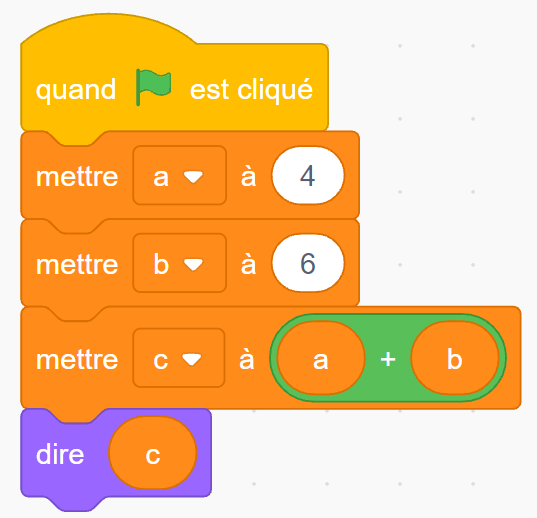
\includegraphics[width=0.5\linewidth]{images/pretest/_Q1.png}
\end{figure}

\begin{enumerate}[label=\alph*)]
    \item c
    \item 4
    \item 6
    \item \textbf{10}
    \item 12
\end{enumerate}
\newpage

\textbf{Q2} (Loop for) * - The program below should display 'Bla Bla Bla Bla Bla' when executed:
\begin{figure}[H]
    \centering
    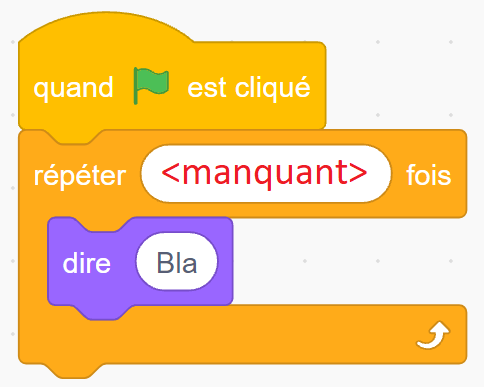
\includegraphics[width=0.45\linewidth]{images/pretest/_Q2.png}
\end{figure}
What value should be given to the missing code? (<manquant>)
\begin{enumerate}[label=\alph*)]
    \item 1
    \item 2
    \item 3
    \item 4
    \item \textbf{5}
\end{enumerate}
\newpage
\textbf{Q3} (conditional) * -
What does the program below display when executed?
\begin{figure}[H]
    \centering
    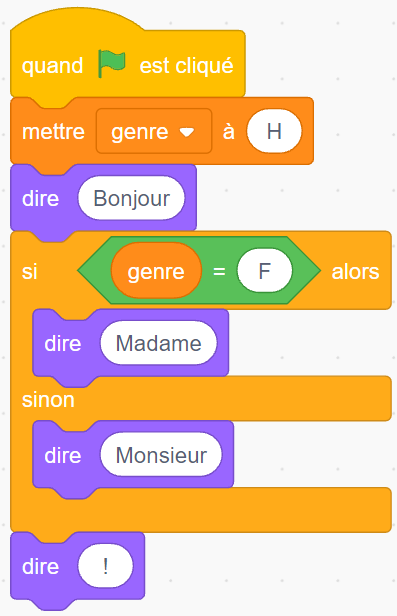
\includegraphics[width=0.5\linewidth]{images/pretest/_Q3.png}
\end{figure}

\begin{enumerate}[label=\alph*)]
    \item Bonjour Madame
    \item Bonjour Monsieur
    \item Bonjour Madame Monsieur !
    \item Bonjour Madame !
    \item \textbf{Bonjour Monsieur !}
\end{enumerate}
\newpage
\textbf{Q4} (variable) ** - 
What does the program below display when executed? For your information, the block * is used to perform multiplication.

\begin{figure}[H]
    \centering
    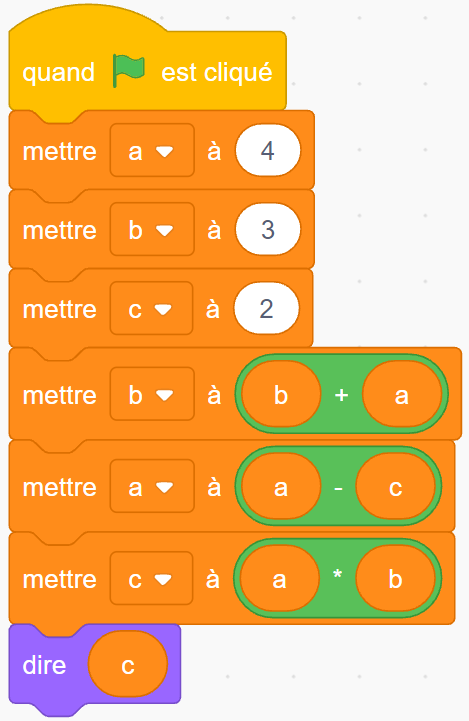
\includegraphics[width=0.5\linewidth]{images/pretest/_Q4.jpg}
\end{figure}

\begin{enumerate}[label=\alph*)]
    \item c
    \item 2
    \item 9
    \item 12
    \item \textbf{14}
\end{enumerate}
\newpage
\textbf{Q5} (for loop) ** - What does the program below display when executed?
\begin{figure}[H]
    \centering
    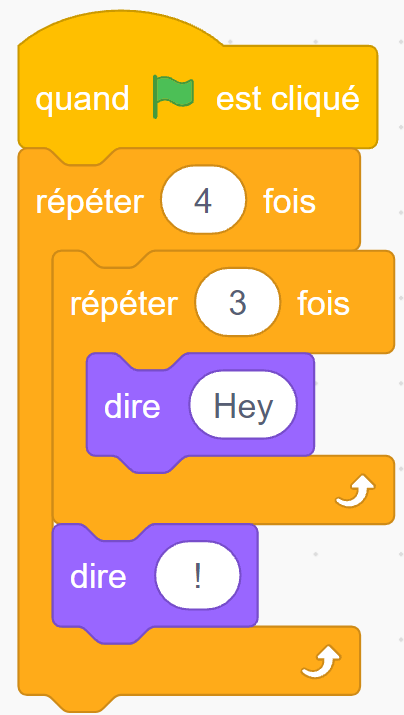
\includegraphics[width=0.35\linewidth]{images/pretest/_Q5.png}
\end{figure}
\begin{enumerate}[label=\alph*)]
    \item \textbf{Hey Hey Hey ! \\
Hey Hey Hey ! \\
Hey Hey Hey ! \\
Hey Hey Hey !}

    \item Hey Hey Hey Hey ! \\
Hey Hey Hey Hey ! \\
Hey Hey Hey Hey !

    \item Hey ! Hey ! Hey ! \\
Hey ! Hey ! Hey ! \\
Hey ! Hey ! Hey ! \\
Hey ! Hey ! Hey !
 
    \item Hey ! Hey ! Hey ! Hey ! \\
Hey ! Hey ! Hey ! Hey ! \\
Hey ! Hey ! Hey ! Hey !

    \item Hey Hey Hey \\
Hey Hey Hey \\
Hey Hey Hey \\
Hey Hey Hey !

\end{enumerate}
\newpage
\textbf{Q6} (conditional)** - 
The program below should display “Adult” when executed:
\begin{figure}[H]
    \centering
    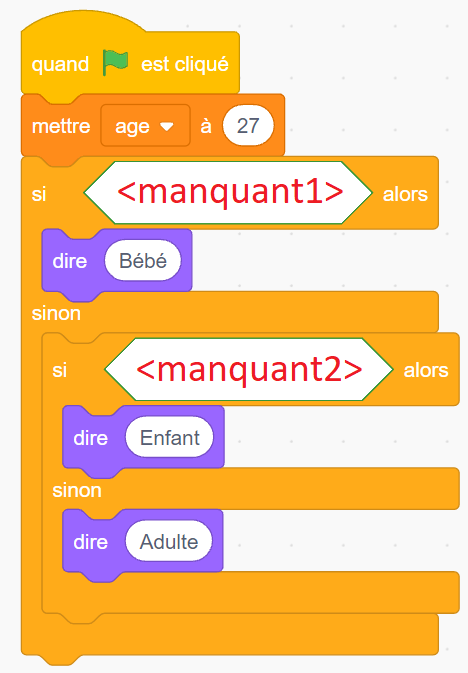
\includegraphics[width=0.55\linewidth]{images/pretest/_Q6.png}
\end{figure}
What is the missing code? (\texttt{<manquant1>} and \texttt{<manquant2>})
\begin{enumerate}[label=\alph*)]
    \item \texttt{<manquant1>}: 
\includegraphics[width=0.2\linewidth]{images/pretest/_Q6_B.png} \texttt{<manquant2>} :   
\includegraphics[width=0.2\linewidth]  {images/pretest/_Q6_C.png}\textbf{Correct answer}
    \item \texttt{<manquant1>} : 
\includegraphics[width=0.2\linewidth]{images/pretest/_Q6_A.png} \texttt{<manquant2>} :   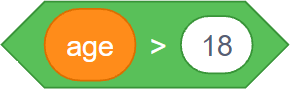
\includegraphics[width=0.2\linewidth]{images/pretest/_Q6_D.png} 
    \item \texttt{<manquant1>} : 
\includegraphics[width=0.2\linewidth]{images/pretest/_Q6_B.png} \texttt{<manquant2>} :   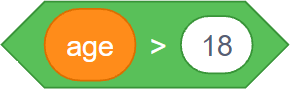
\includegraphics[width=0.2\linewidth]{images/pretest/_Q6_D.png} 
    \item \texttt{<manquant1>} : 
\includegraphics[width=0.2\linewidth]{images/pretest/_Q6_A.png} \texttt{<manquant2>} :   
\includegraphics[width=0.2\linewidth]{images/pretest/_Q6_C.png} 
    \item \texttt{<manquant1>} : 
\includegraphics[width=0.2\linewidth]{images/pretest/_Q6_E.png} \texttt{<manquant2>} :   
\includegraphics[width=0.2\linewidth]{images/pretest/_Q6_E.png} 
\end{enumerate}

\newpage
\textbf{Q7} (variable) *** - The program below must calculate the perimeter of a circle using the following formula:
$P = 2 \times \pi \times R $ where $\pi \approx 3.14$ and $R$ is the radius of the circle.
\begin{figure}[H]
    \centering
    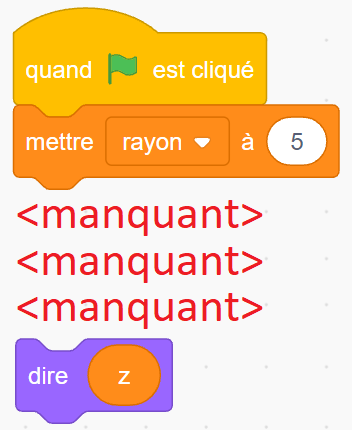
\includegraphics[width=0.4\linewidth]{images/pretest/_Q7.png}
\end{figure}
What is the missing code? (\texttt{<manquant>})
\begin{enumerate}[label=\alph*)]
    \item 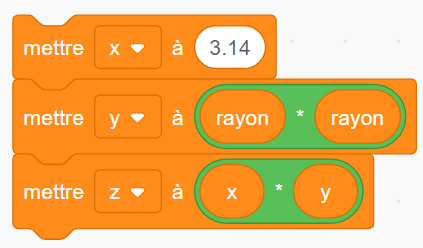
\includegraphics[width=0.4\linewidth]{images/pretest/_Q7_A.png} \textbf{Correct answer}
    \item 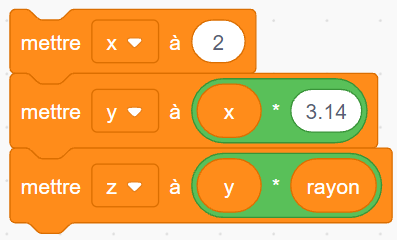
\includegraphics[width=0.4\linewidth]{images/pretest/_Q7_B.png}
    \item 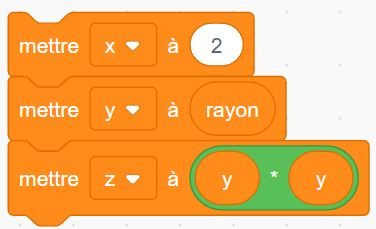
\includegraphics[width=0.4\linewidth]{images/pretest/_Q7_C.png}
    \item 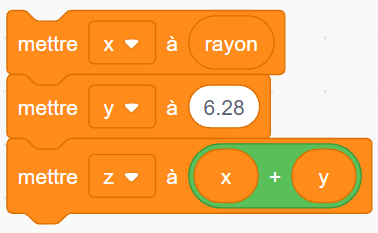
\includegraphics[width=0.4\linewidth]{images/pretest/_Q7_D.png}
    \item 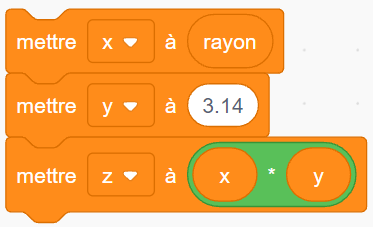
\includegraphics[width=0.4\linewidth]{images/pretest/_Q7_E.png}
\end{enumerate}
\newpage
\textbf{Q8}
(for loop) *** - What does the program below display when executed?
\begin{figure}[H]
    \centering
    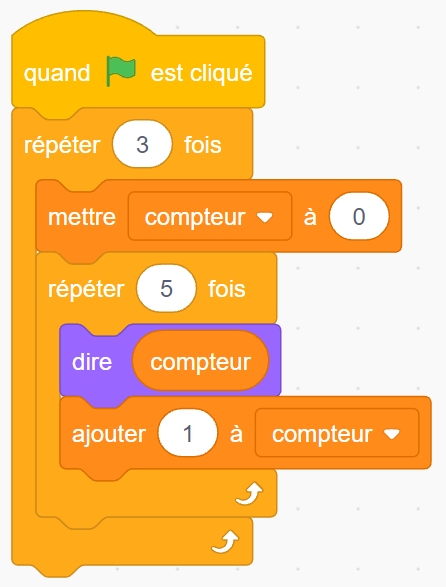
\includegraphics[width=0.5\linewidth]{images/pretest/_Q8.png}
\end{figure}

\begin{enumerate}[label=\alph*)]
    \item It displays 15 times the word “counter”
    \item It displays 3 times the numbers from 1 to 5
    \item It displays 3 times the numbers from 1 to 6
    \item \textbf{It displays 3 times the numbers from 0 to 4}
    \item It displays 3 times the numbers from 0 to 5
\end{enumerate}
\newpage
\textbf{Q9} (conditional) *** -
What does the program below display when executed?
\begin{figure}[H]
    \centering
    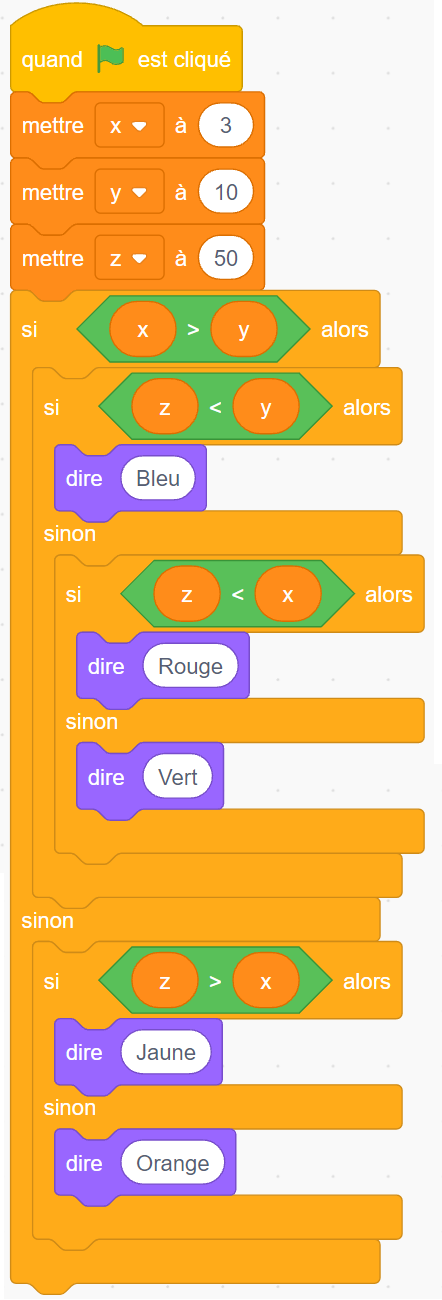
\includegraphics[width=0.4\linewidth]{images/pretest/_Q9.png}
\end{figure}

\begin{enumerate}[label=\alph*)]
    \item Bleu
    \item Rouge
    \item Vert
    \item \textbf{Jaune}
    \item Orange
\end{enumerate}
\newpage
\section{Post-test}
\textbf{Q1} (variable) * - What is the display produced by the program below when executed?
\begin{figure}[H]
    \centering
    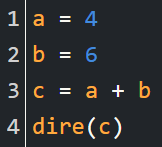
\includegraphics[width=0.25\linewidth]{images/posttest/_Q1.png}
\end{figure}

\begin{enumerate}[label=\alph*)]
    \item c
    \item 4
    \item 6
    \item \textbf{10}
    \item 12
\end{enumerate}
\newpage
\textbf{Q2} (Loop for) * - The program below should display 'Bla Bla Bla Bla Bla' when executed:
\begin{figure}[H]
    \centering
    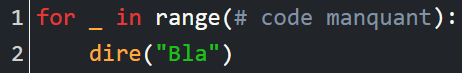
\includegraphics[width=0.7\linewidth]{images/posttest/_Q2.png}
\end{figure}
What value should be given to the missing code? (<manquant>)
\begin{enumerate}[label=\alph*)]
    \item 1
    \item 2
    \item 3
    \item 4
    \item \textbf{5}
\end{enumerate}
\newpage
\textbf{Q3} (conditional) * -
What does the program below display when executed?
\begin{figure}[H]
    \centering
    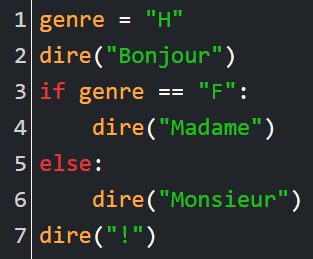
\includegraphics[width=0.45\linewidth]{images/posttest/_Q3.png}
\end{figure}

\begin{enumerate}[label=\alph*)]
    \item Bonjour Madame
    \item Bonjour Monsieur
    \item Bonjour Madame Monsieur !
    \item Bonjour Madame !
    \item \textbf{Bonjour Monsieur !}
\end{enumerate}
\newpage
\textbf{Q4} (variable) ** - 
What does the program below display when executed? For your information, the operator * is used to perform multiplication.

\begin{figure}[H]
    \centering
    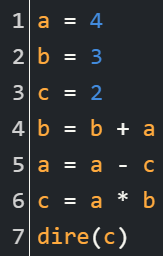
\includegraphics[width=0.25\linewidth]{images/posttest/_Q4.png}
\end{figure}

\begin{enumerate}[label=\alph*)]
    \item c
    \item 2
    \item 9
    \item 12
    \item \textbf{14}
\end{enumerate}
\newpage
\textbf{Q5} (for loop) ** - What does the program below display when executed?
\begin{figure}[H]
    \centering
    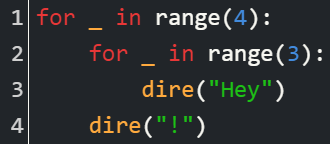
\includegraphics[width=0.5\linewidth]{images/posttest/_Q5.png}
\end{figure}
\begin{enumerate}[label=\alph*)]
    \item \textbf{Hey Hey Hey ! \\
Hey Hey Hey ! \\
Hey Hey Hey ! \\
Hey Hey Hey !}

    \item Hey Hey Hey Hey ! \\
Hey Hey Hey Hey ! \\
Hey Hey Hey Hey !

    \item Hey ! Hey ! Hey ! \\
Hey ! Hey ! Hey ! \\
Hey ! Hey ! Hey ! \\
Hey ! Hey ! Hey !
 
    \item Hey ! Hey ! Hey ! Hey ! \\
Hey ! Hey ! Hey ! Hey ! \\
Hey ! Hey ! Hey ! Hey !

    \item Hey Hey Hey \\
Hey Hey Hey \\
Hey Hey Hey \\
Hey Hey Hey !

\end{enumerate}
\newpage
\textbf{Q6} (conditional)** - 
The program below should display “Adult” when executed:
\begin{figure}[H]
    \centering
    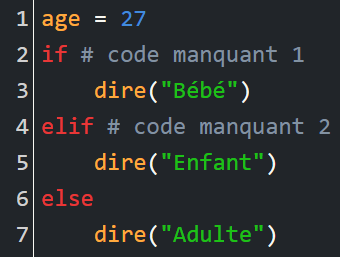
\includegraphics[width=0.5\linewidth]{images/posttest/_Q6.png}
\end{figure}
What is the missing code? (\# code manquant 1 and \# code manquant 2)
\begin{enumerate}[label=\alph*)]
    \item \textbf{manquant1 : 
\includegraphics[width=0.2\linewidth]{images/posttest/_Q6_B.png} manquant2 :   
\includegraphics[width=0.2\linewidth]{images/posttest/_Q6_C.png} }    
    \item manquant1 : 
\includegraphics[width=0.2\linewidth]{images/posttest/_Q6_A.png} manquant2 :   
\includegraphics[width=0.2\linewidth]{images/posttest/_Q6_D.png} 
    \item manquant1 : 
\includegraphics[width=0.2\linewidth]{images/posttest/_Q6_B.png} manquant2 :   
\includegraphics[width=0.2\linewidth]{images/posttest/_Q6_D.png} 
    \item manquant1 : 
\includegraphics[width=0.2\linewidth]{images/posttest/_Q6_A.png} manquant2 :   
\includegraphics[width=0.2\linewidth]{images/posttest/_Q6_C.png} 
    \item manquant1 : 
\includegraphics[width=0.2\linewidth]{images/posttest/_Q6_E.png} manquant2 :   
\includegraphics[width=0.2\linewidth]{images/posttest/_Q6_E.png} 
\end{enumerate}
\newpage
\textbf{Q7} (variable) *** - The program below must calculate the perimeter of a circle using the following formula:
$P = 2 \times \pi \times R $ where $\pi \approx 3.14$ and $R$ is the radius of the circle.
\begin{figure}[H]
    \centering
    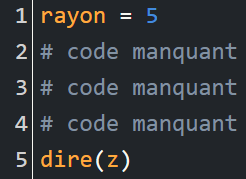
\includegraphics[width=0.4\linewidth]{images/posttest/_Q7.png}
\end{figure}
What is the missing code? (\# code manquant)
\begin{enumerate}[label=\alph*)]
    \item 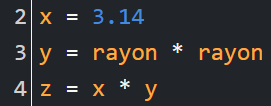
\includegraphics[width=0.4\linewidth]{images/posttest/_Q7_A.png} \textbf{Correct answer}
    \item 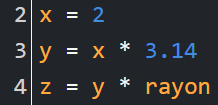
\includegraphics[width=0.35\linewidth]{images/posttest/_Q7_B.png}
    \item 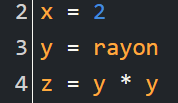
\includegraphics[width=0.3\linewidth]{images/posttest/_Q7_C.png}
    \item 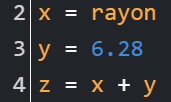
\includegraphics[width=0.3\linewidth]{images/posttest/_Q7_D.png}
    \item 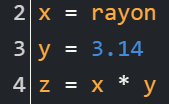
\includegraphics[width=0.3\linewidth]{images/posttest/_Q7_E.png}
\end{enumerate}
\newpage
\textbf{Q8}
(for loop) *** - What does the program below display when executed?
\begin{figure}[H]
    \centering
    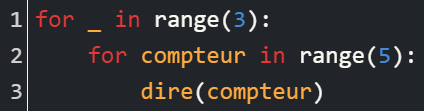
\includegraphics[width=0.7\linewidth]{images/posttest/_Q8.png}
\end{figure}

\begin{enumerate}[label=\alph*)]
    \item It displays 15 times the word “counter”
    \item It displays 3 times the numbers from 1 to 5
    \item It displays 3 times the numbers from 1 to 6
    \item \textbf{It displays 3 times the numbers from 0 to 4}
    \item It displays 3 times the numbers from 0 to 5
\end{enumerate}
\newpage
\textbf{Q9} (conditional) *** -
What does the program below display when executed?
\begin{figure}[H]
    \centering
    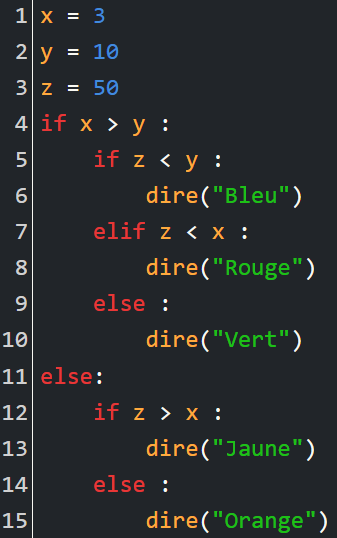
\includegraphics[width=0.55\linewidth]{images/posttest/_Q9.png}
\end{figure}

\begin{enumerate}[label=\alph*)]
    \item Bleu
    \item Rouge
    \item Vert
    \item \textbf{Jaune}
    \item Orange
\end{enumerate}
\newpage
[ONLY FOR EXPERIMENTAL GROUP]\\
\\
\textbf{QA} (qualitative)
Did you find the tutor helps useful for progressing in the game?
Rate from “not at all” (0) to “very much” (100) by moving the slider.\\
\\
\textbf{QB} (qualitative)
Would you like to have more helps from tutors in the future?
Rate from “not at all” (0) to “very much” (100) by moving the slider.


\end{document}  % End of the document content